\begin{tikzpicture}
  \begin{scope}[yshift=0cm]
    \begin{scope}[xshift=0cm]
      \node [mybox] (box){
        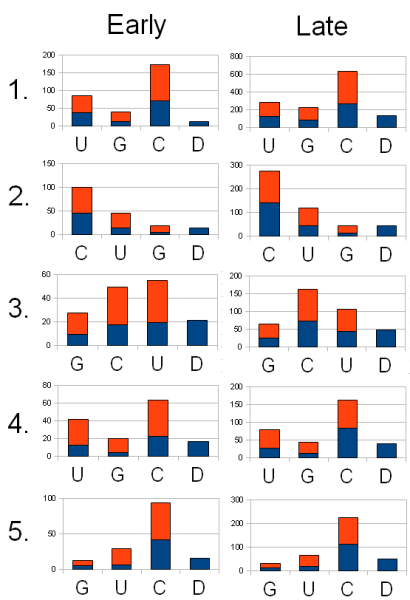
\includegraphics[width=0.35\textwidth]{../figures/whichisthecomputer.png}
      };
    \end{scope}
  \end{scope}
  \begin{scope}[yshift=0.15\textwidth]
    \begin{scope}[xshift=0.5\textwidth]
      \node [mybox] (box) [text width=0.5\textwidth]{
        This talk is based on the current latest blog post by Tim Gowers
      };
    \end{scope}
  \end{scope}
  \begin{scope}[yshift=0.0\textwidth]
    \begin{scope}[xshift=0.5\textwidth]
      \node [mybox] (box) [text width=0.5\textwidth]{
        Results taken after revealing that one solution was produced by a computer
      };
    \end{scope}
  \end{scope}
  \begin{scope}[yshift=-0.15\textwidth]
    \begin{scope}[xshift=0.5\textwidth]
      \node [mybox] (box) [text width=0.5\textwidth]{
        Computer identified $\sim50\%$ of the time, but undergraduate a strong contender
      };
    \end{scope}
  \end{scope}
\end{tikzpicture}
